

\documentclass[11pt]{article}
%Gummi|065|=)
\title{\textbf{Sistemas Electronicos De Interfaz\\-Convertidores-
}}
\author{Miguel Angel Xamie Diaz Fuentes}
\date{}
\usepackage{graphicx}
\begin{document}

\maketitle

\section{Convertidores CC-CA}
El convertidor de CC/CA tambien conocido como inversor, es un circuito que convierte una fuente de CC en tension de CA sinusoidal para suministrar cargas de CA, controlar motores de CA o incluso conectar dispositivos de CC conectados a la red. Al igual que un convertidor CC/CC, la entrada de un inversor puede ser una fuente directa como una bateria, una celda solar, o una pila de combustible o puede provenir de un enlace de CC intermedio que puede suministrarse desde una fuente de CA.\\\\ Generalmente, los inversores se pueden clasificar segun su salida de CA como monofasicos o trifasicos y tambien como convertidores de puente medio o completo.\\\\ De Lorenzo ha diseñado dos configuraciones para implementar esta categoria. Una configuracion para cubrir los inversores con control PWM y otra configuracion para explicar las propiedades del circuito convertidor de frecuencia.\\ Respecto al convertidor de frecuencia y porque es dificil cambiar la frecuencia de una onda sinusoidal de CA en modo CA, la primera tarea de un convertidor de frecuencia es convertir la onda a CC ya que es relativamente facil manipular la CC para hacerla parecer como CA. Los tres componentes principales de todos los convertidores de frecuencia son: rectificador, bus de CC e inversor.\\\\ 
El termino "Inversor" tambien se puede utilizar para referirse a un grupo "rectificador-inversor", alimentando por corriente alterna y utilizado para variar el voltaje y la frecuencia de la corriente alterna en la salida en funcion de la corriente de entrada (por ejemplo, para la alimentacion de particulares maquinas de operacion). Los inversores mas comunes utilizados para alimentar cargas de corriente alterna son de tres tipos: inversores de onda cuadrada (adecuados para cargas puramente resistivas), inversores de sinusoidal modificada (adecuados para cargas resistivas y capacitivas, con cargas inductivas pueden producir ruido) e inversor de onda sinusoidal pura (adecuados para todo tipo de cargas porque reproducen fielmente una onda senoidal igual a la de nuestra red electrica domestica).
\subsection{De Tension}

\subsection{De Corriente}
\subsubsection{Monofasico}
Un inversor simple consta de un oscilador que controla a un transistor, el cual se utiliza para interrumpir la corriente entrante y generar una onda senoidal.
\begin{figure}[htp]
\centering
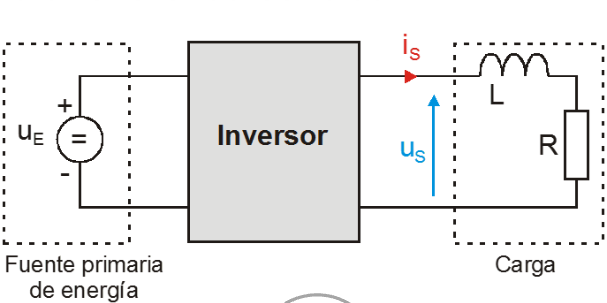
\includegraphics[scale=0.50]{/home/monkeydmigue/Documentos/LaTex/Gummi/Circuito monofasico.png}
\caption{Estructura Monofasica}
\label{}
\end{figure}
\pagebreak
\subsubsection{Semi-Puente}
Tensión máxima que deben soportar los interruptores de potencia: UB, más las sobretensiones que originen los circuitos prácticos.\\\\Tension maxima en la carga UB/2, por tanto para igual potencia corrientes mas elevadas que en el puente completo.\\\\Topologia adecuada para tension en la bateria alta y potencia en la carga media.
\begin{figure}[htp]
\centering
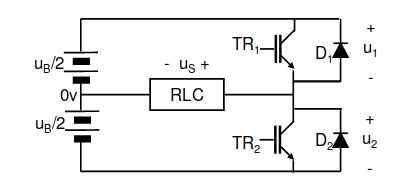
\includegraphics[scale=0.80]{/home/monkeydmigue/Documentos/LaTex/Gummi/Medio Puente (Half Bridge).png}
\caption{Medio Puente}
\label{}
\end{figure}
\begin{figure}[htp]
\centering
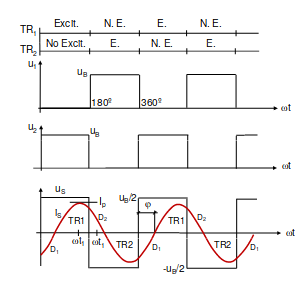
\includegraphics[scale=0.80]{/home/monkeydmigue/Documentos/LaTex/Gummi/Medio Puente (Half Bridge)2.png}
\caption{Medio Puente}
\label{}
\end{figure}
\pagebreak
\subsubsection{Puente Completo}
Tension maxima que deben soportar los interruptores de potencia: UB, mas las sobretensiones que originen los circuitos practicos.\\\\Tension maxima en la carga UB,por tanto para igual potencia corrientes mas bajas  que en el medio puente.\\\\Topologia adecuada para tensión en la bateria alta y potencia en la carga alta.\\\\Doble nº de interruptores de potencia que en el medio puente y que en el Push-Pully de gobierno más complejo por no tener un terminal referido a masa, (T1 y T3).

\begin{figure}[htp]
\centering 

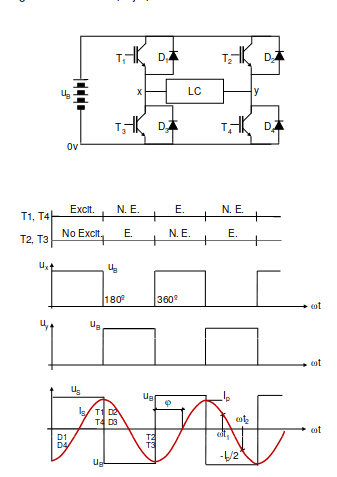
\includegraphics[scale=0.80]{/home/monkeydmigue/Documentos/LaTex/Gummi/Puente Completo (Full Bridge).png}
\caption{Puente Completo (Full Bridge)}
\label{}
\end{figure}



\pagebreak

\subsubsection{Push-Pull}
Tension maxima que deben soportar los interruptores de potencia: UB, mas las sobretensiones que originen los   circuitos practicos, que en este caso seran mayores debido a la inductancia de dispersion del transformador.\\\\Tension maxima en la carga UB.B\\\\El transformador de toma media tiene un factor de utilizacion bajo en el primario y empeora bastante el rendimiento de los circuitos practicos. No es aconsejable utilizar esta topologia para potencias de mas de 10kVA.\\\\Solo utiliza dos interruptores de potencia y ambos estan referidos a masa y por tanto su gobierno es sencillo.
\begin{figure}[htp]
\centering
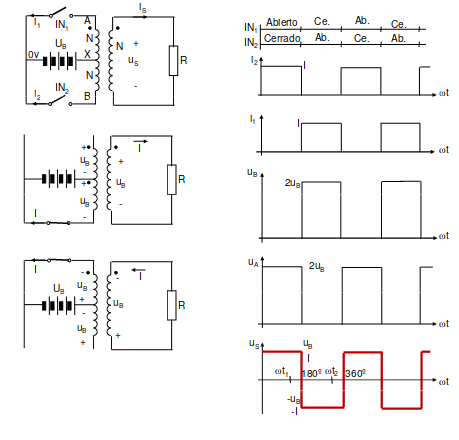
\includegraphics[scale=0.70]{/home/monkeydmigue/Documentos/LaTex/Gummi/Push Pull.png}
\caption{Push Pull}
\label{}
\end{figure}
\pagebreak

\subsubsection{Trifasico}
- Aplicaciones de Alta Potencia.\\\\- Acoplando tres inversores trifasicos.\\\\- Las señales de disparo deben estar desfasadas 120 (grados) entre si.\\\\- Los secundarios de los transformadores se colocan en estrella debido a que se eliminan los armonicos de triples.
\begin{center}
\begin{figure}[htp]
\centering
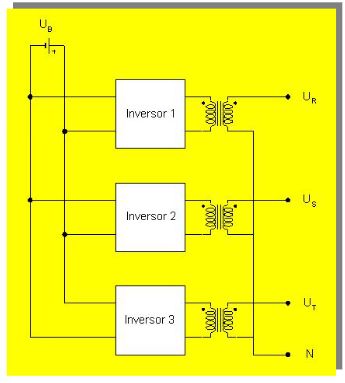
\includegraphics[scale=0.70]{Convertidor Trifasico.png}
\caption{Convertidor Trifasico}
\label{}
\end{figure}
\end{center}

\subsubsection{En Estrella}
Si los devanados de fase de un generador o consumidor se conectan de modo que los finales de los devanados se unan en un punto comun, y los comienzos de estos sean conectados a los conductores de la línea, tal conexion se llama conexion en estrella y se designa con el símbolo Y.\\\\
Durante el servicio por el conductor neutro pasa una corriente igual a la suma geometrica de tres corrientes $I_A$, $I_B$ e $I_C$ que son las corrientes de fase, es decir: $I_N$ y el punto neutro se llaman tensiones de fase y se designan con $U_A$, $U_B$, $U_C$ o en forma general con $U_f$. A menudo se establecen de antemano las magnitudes de la fuerza electromotriz (fem) en los devanados de fase del generador, designandose estas con $E_A$, $E_B$, $E_C$ o $E_f$. Despreciando la resistencia de los devanados del generador, se puede escribir: $E_A$ = $U_A$; $E_B$ = $U_B$; $E_C$ = $U_C$; $E_f$ = $U_f$ Las tensiones medidas entre los comienzos de las fases A y B, B y C, C y A del generador o consumidor se llaman tensiones compuestas y se designan por $U_AB$, $U_BC$, $U_CA$ o en forma general con $U_comp$ o tensión de línea $U_L$.
\begin{center}
\begin{figure}[htp]
\centering
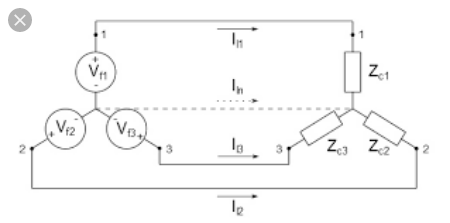
\includegraphics[scale=0.70]{Circuito Estrella.png}
\caption{Estrella}
\label{}
\end{figure}
\end{center}


\subsubsection{En Delta}
Es de mucha utilidad el poder obtener las corrientes de fase a partir de las corrientes de linea y viceversa en problemas que involucren cargas o fuentes en forma de delta. La razon es que cuando en un circuito trifasico tenemos una carga en forma de delta no podemos obtener un circuito monofasico equivalente ya que no hay linea neutra. Como un circuito monofasico es mas facil de resolver que uno trifasico lo mejor en este caso es transformar la delta utilizando transformaciones delta-Y a una Y, posteriormente ya que se tiene la carga y la fuente en forma de Y se puede obtener el circuito equivalente monofasico como se explico anteriormente y asi obtener la corriente de linea. Una vez que obtenemos esta corriente de linea es posible saber en base a esta cuánto vale la corriente en cada una de las ramas de la delta y por lo tanto se da respuesta al problema inicial.
\begin{center}
\begin{figure}[htp]
\centering
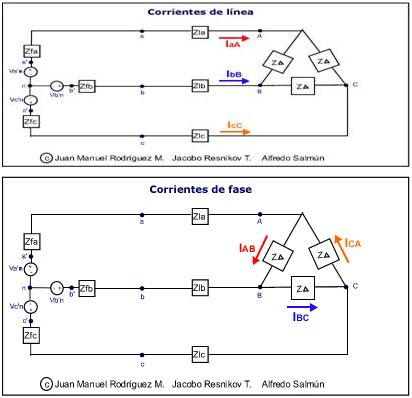
\includegraphics[scale=0.70]{Conexion delta.png}
\caption{Delta}
\label{}
\end{figure}
\end{center}


\subsection{Forma de Onda de Salida}
\subsubsection{Cuadrada y Casi cuadrada}
Son mas baratos, pero normalmente generan mas problemas de funcionamiento. Producen armonicos (frecuencias multiplos de la frecuencia de red) que generan interferencias. No son aptos para motores de induccion. Se utilizaran unicamente cuando se desea corriente alterna para alimentar un televisor, un ordenador o un aparato electrico.\\Se usa principalmente para la generacion de pulsos eléctricos que son usados como señales (1 y 0) que permiten ser manipuladas fácilmente, un circuito electrónico que genera ondas cuadradas se conoce como generador de pulsos,  
\begin{center}
\begin{figure}[htp]
\centering
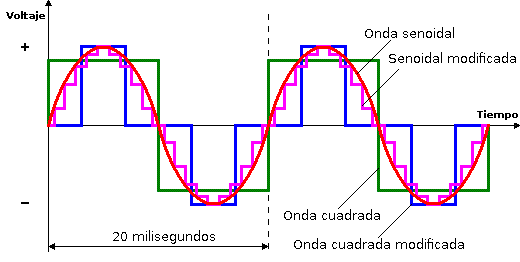
\includegraphics[scale=0.50]{Onda cuadrada y casi cuadrada.png}
\caption{Onda Cuadrada y Casi Cuadrada}
\label{}
\end{figure}
\end{center}
\subsubsection{Moduladas}
Senales portadoras: es una forma de onda, que es modulada por una senal que se quiere transmitir.\\
Al modular una senal desplazamos su contenido en frecuencia, ocupando un cierto ancho de banda alrededor de la frecuencia de la onda portadora, permitiendonos multiplexar en frecuencia varias senales simplemente utilizando diferentes ondas portadoras y conseguir asi un uso más eficiente.\\\\
Señal moduladora: Es la señal que contiene la información a transmitir.\\
La modulacion es la adicion de informacion a una senal electronica u optica de transmision principal pudiendo ser aplicada desde una corriente directa como onda principal (apagandola y encendiendola), a una corriente alterna y a senales opticas como las usadas en fibra optica.\\\\
Modulacion de amplitud: consiste en hacer variar la amplitud de la onda portadora de forma que esta cambie de acuerdo con las variaciones de nivel de la senal moduladora, que es la informacion que se va a transmitir.\\
La AM es usada en la radiofonia, en las ondas medias y en las ondas cortas. Permite llegar a mas lugares, pero con una calidad de sonido menor.\\\\
Modulacion de frecuencia: es una modulacion angular que transmite informacion a traves de una onda portadora variando su frecuencia.\\
La FM permite llegar a menos sitios, pero con menor nitidez de sonido.\\\\
Modulacion de fase (PM): Es el caso de modulacion donde tanto las senales de transmision como las senales de datos son analogicas. Es un tipo de modulacion exponencial al igual que la modulacion de frecuencia. Se caracteriza porque la fase de la onda portadora varía directamente de acuerdo con la senal modulada.
\begin{figure}[htp]
\centering
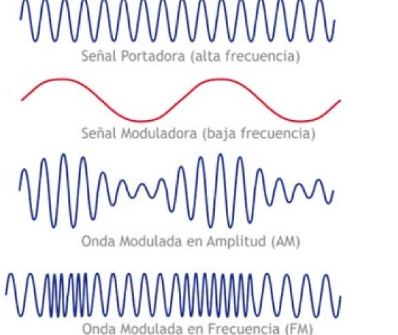
\includegraphics[scale=0.60]{Ondas Moduladas.png}
\caption{Ondas Moduladas}
\label{}
\end{figure}

\subsubsection{Multi-Nivel}
La idea de estos inversores consiste en sumar las ondas cuasi cuadradas de salida obtenidas con varios inversores. Para esto se conectan en serie las salidas de dichos inversores.\\
Se genera en cada inversor una onda casi cuadrada, con diferentes angulos de disparo y de conduccion y luego se suman dichas ondas en el secundario del transformador, consiguiendose asi una onda resultante mas parecida a una onda sinusoidal.
Las ondas generadas en los diferentes inversores estan centradas en el pico de la onda sinusoidal que se quiere construir. A medida que se aumenta la cantidad de inversores, con sus salidas conectadas en serie, ira aumentando la cantidad de escalones, consiguiendose una forma de onda cada vez mas semejante a una onda sinusoidal.
\begin{figure}[htp]
\centering
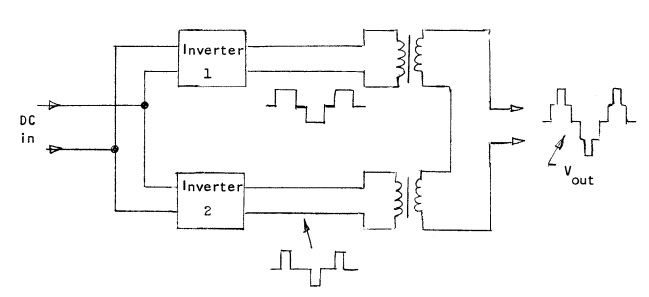
\includegraphics[scale=0.70]{Multinivel.png}
\caption{Multinivel}
\label{}
\end{figure}


\section{Convertidores CA-CA}
La  electronica de potencia ac-ac convertidor de corriente alterna, en forma generica, acepta de energia electrica de un sistema y la convierte para su entrega a otro sistema de corriente alterna con formas de onda de amplitud diferente, frecuencia y fase. Pueden ser de una o tres fases tipos en funcion de sus clasificaciones de poder. La ac -ac convertidores empleados para variar la tension eficaz a traves de la carga constante frecuencia son conocidos como  controladores  o  reguladores  de  voltaje  de  ca de ca.  El  control  de  voltaje  se  logra  mediante:  (i)  control  de fase en virtud de la conmutacion fisica que utiliza pares de controlado desilicio rectificadores (SCR) o triac, o (ii) por   el   control de   compensacion   con   arreglo   a -forzada   conmutacion   con   conmutadores   controlados completamente auto-conmutados como Tiristores Puerta Apagar-(OTG), transistores de potencia, Los transistores bipolares  de  puerta  aislada  (IGBT),  controlado  por  MOS  Tiristores  (MCT),  etc   ac -convertidores  de  corriente alterna  en  la  que  corriente  alterna  en  una  frecuencia  se  convierte  directamente  en  corriente  alterna  en  otra frecuencia  sin  ningún  tipo  de  conversión de  corriente  continua  intermedios  enlace  se  conocen  como  ciclo convertidores,  la  mayoría  de  los  que  utilizan  naturalmente  conmutados  SCR  para  su  funcionamiento  cuando  la frecuencia de salida máxima se limita a una fraccion del frecuencia de entrada.
\section{Variadores de CA}
Un variador de frecuencia es un sistema para el control de la velocidad rotacional de un motor de corriente alterna (AC) por medio del control de la frecuencia de alimentaciOn suministrada al motor. Un variador de frecuencia es un caso especial de un variador de velocidad. Los variadores de frecuencia son tambien conocidos como drivers de frecuencia ajustable (AFD), drivers de CA o microdrivers. Dado que la tension (o voltaje) se hace variar a la vez que la frecuencia, a veces son llamados drivers VVVF (variador de voltaje variador de frecuencia).
\begin{figure}[htp]
\centering
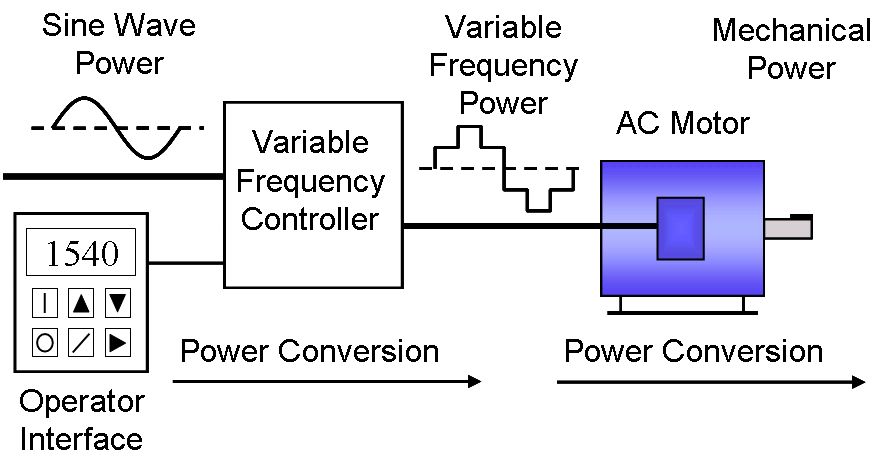
\includegraphics[scale=0.30]{Variadores de CA.png}
\caption{Variador de CA}
\label{}
\end{figure}

\pagebreak
\subsection{Ciclo Controladores}
SI un conmutador con tiristores se conecta entre la fuente AC y la carga, se puede controlar el flujo de potencia mediante la variacion del voltaje RMS aplicado a la carga; este tipo de circuitos de potencia son conocidos como controladores de voltaje alterno (Controladores AC-AC).
\begin{figure}[htp]
\centering
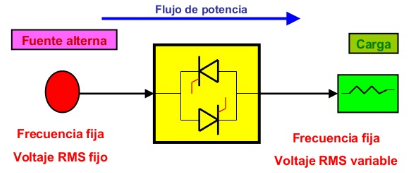
\includegraphics[scale=0.60]{Ciclo controladores.png}
\caption{Ciclo Controladores}
\label{}
\end{figure}
\subsection{Convertidores Matriciales}
El CM es un convertidor CA-CA trifasico que se considera de la nueva generacion de variadores de velocidad integrados, dado que no requiere de componentes que almacenen energia, como capacitores para bus de CD, lo que permite reducir el volumen del convertidor y alargar la vida util del mismo. Este puede ser implementado de manera modular, haciendolo aun mas compacto. La transferencia de energia es bi-direccional y la conversion de potencia es directa, es decir, no existen etapas intermedias dentro del CM. Las corrientes de entrada son senoidales generando un factor de potencia alto, y que puede ser controlado independientemente de la carga que sea conectada.
\begin{figure}[htp]
\centering
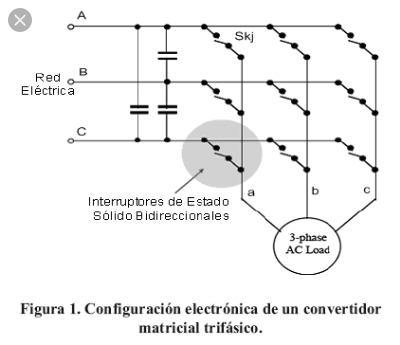
\includegraphics[scale=0.30]{Controladores Matriciales.png}
\caption{Controladores Matriciales}
\label{}
\end{figure}

\section{Convertidores CA-CD}

Un  convertidor  de  corriente  alterna  a  corriente  directa  parte  de  un  rectificador  de  onda  completa.  Su  carga  puede  ser  puramente  resistiva,  figura  1.1a.  La  forma  de  onda  de  salida  del  rectificador  se  muestra  en  la  figura  1.1b.  Al  agregarle  a  este  rectificador  un  capacitor en paralelo tal como lo indica la figura 1.2a, el convertidor se comporta como un filtro ya que se produce un voltaje a la salida que es esencialmente continuo, 1.2b.\\\\
El  convertidor  CA-CD  nos  proporciona  una  señal  de  salida  rectificada  (casi  constante)  de  valor  $V_m$,  donde  $V_m$  es  igual  al  valor  pico  del  voltaje  de  entrada  como  se  muestra  en  la  figura  1.2b.  Este  voltaje  casi  constante  presenta  una  variación  de  $V_0$.  Este  valor  se  puede  considerar  muy  pequeño  y  de  esta  manera  encontrar  el  valor  del  resistor  y  del capacitor para un valor de voltaje directo deseado.
\begin{figure}[htp]
\centering
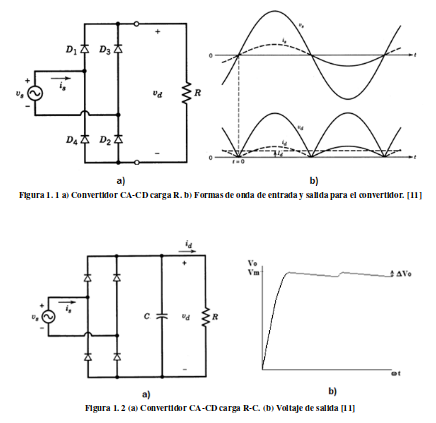
\includegraphics[scale=0.71]{Convertidor ca-cd.png}
\caption{Convertidor CA-CD}
\label{}
\end{figure}
\subsection{No controlados}
Los rectificadores o convertidores de corriente se caracterizan por transformar la corriente alterna en continua. De esta manera permiten la conversion directa desde un circuito alimentado con voltaje  alterno,  poder  alimentar  a  la  carga  con  corriente  continua.  Los  rectificadores  no  controlados  estan formados exclusivamente por diodos, no necesitando circuitos de mando, por lo que los diodos conmutan de manera natural forzados por la fuente de alimentacion.

\subsection{Controlados}
Los rectificadores controlados emplean el tiristor o SCR(rectificador controlado de silicio) como dispositivo de control.\\
El tiristor es un semiconductor que presenta dos estados estables: en uno conduce, y en otro esta en corte(bloqueo directo, bloqueo inverso y conduccion directa).\\
El objetivo del tiristor es retardar la entrada en conduccion del mismo, ya que como se sabe, un tiristor se hace conductor no solo cuando la tension en sus bornes se hace positiva (tension de ánodo mayor que tensión de catodo), sino cuando siendo esta tension positiva, se envia un impulso de cebado a puerta.\\
El parametro principal de los rectificadores controlados es el angulo de retardo, a .\\
En los rectificadores controlados se controla el cebado del tiristor y su bloqueo es normalmente natural.

\section{Convertidores CD-CD (CC-CC)}
Se llama convertidor DC-DC a un dispositivo que transforma corriente continua de una tension a otra. Suelen ser reguladores de conmutacion, dando a su salida una tension regulada y, la mayoria de las veces con limitación de corriente. Se tiende a utilizar frecuencias de conmutacion cada vez mas elevadas porque permiten reducir la capacidad de los condensadores, con el consiguiente beneficio de volumen, peso y precio. 
\subsection{Estructuras Basicas Sin Aislamiento}
En cuanto a la corriente galvanica, se produce por contacto entre dos mentales, normalmente por el medio ambiente o en ambientes salinos. Existen medios que reducen este efecto y se puede encontrar abundante informacion al respecto.\\
Un tipo de corriente que, ademas de continua, es ininterrumpida y de intensidad constante. A esta corriente se la denomina galvanica. En cuanto a sus caracteristicas fisicas, la corriente galvanica es de baja tension (60-80 V) y baja intensidad, como maximo 200 mA. Se le denomina tambien constante, porque mantiene su intensidad fija durante el tiempo de aplicacion.
\begin{figure}[htp]
\centering
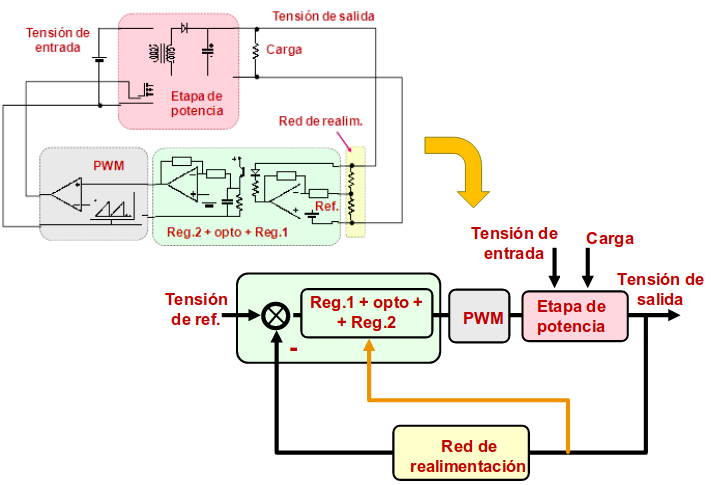
\includegraphics[scale=0.40]{Convertidor SIn Aislamiento.png}
\caption{Convertidor CC-CC Sin Aislamiento}
\label{}
\end{figure}
\subsection{Reductor (Buck)}
El convertidor Buck (o reductor) es un convertidor de potencia, DC/DC sin aislamiento galvanico, que obtiene a su salida una tension menor que a su entrada. El diseno es similar a un convertidor elevador o Boost, tambien es una fuente conmutada con dos dispositivos semiconductores (transistor S y diodo D), un inductor L y opcionalmente un condensador C a la salida.\\\\
La forma mas simple de reducir una tension continua (DC) es usar un circuito divisor de tension, pero los divisores gastan mucha energia en forma de calor. Por otra parte, un convertidor Buck puede tener una alta eficiencia (superior al (95 por ciento) con circuitos integrados) y autoregulacion.\\\\
El funcionamiento del conversor Buck es sencillo, consta de un inductor controlado por dos dispositivos semiconductores los cuales alternan la conexion del inductor bien a la fuente de alimentacion o bien a la carga. 
\begin{figure}[htp]
\centering
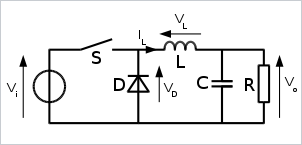
\includegraphics[scale=0.60]{Reductor Buck.png}
\caption{Reductor Buck}
\label{}
\end{figure}

\subsubsection{Directo Forward}
Funciona como el convertidor BUCK pero tiene un transformador que realiza las funciones de aislante de la entrada y la salida pudiendo realizar múltiples salida y de mayor tensión que la entrada dependiendo del devanado del secundario del transformador.
\subsubsection{Directo Forward con 2 interruptores}
Este   circuito   tiene   la   caracteristica   de   poseer   dos   diodos   y   dos   interruptores    para    conectar    y    desconectar    el    devanado    primario    del    transformador  a  la  fuente  de  entrada,  figura  1-7.  Este  circuito  funciona  de  manera similar al Forward convencional.Cuando   los   interruptores   que   funcionan   de   manera   simultanea   no   conducen, los dos diodos interconectan la fuente de entrada con el primario del transformador,  pero  con  polaridad  inversa,  restableciendo  automaticamente  al  devanado primario.
\begin{figure}[htp]
\centering
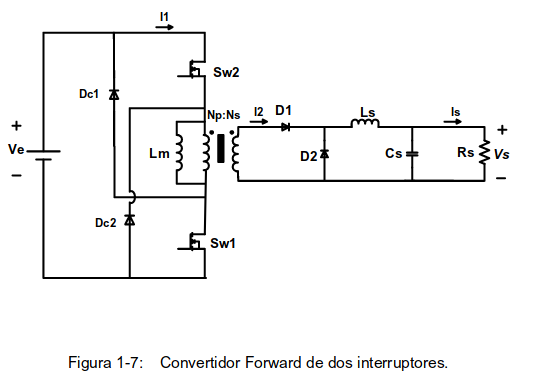
\includegraphics[scale=0.31]{Con 2 interruptores.png}
\caption{Diagrama}
\label{}
\end{figure}
\subsubsection{Estructuras de 2 y 4 cuadrantes sin aislamiento}
\subsubsection{Reversible en Corriente}
En la aplicacion a una maquina de corriente continua, por ejemplo, la alimentacion con reversibilidad de corriente significaria que la maquina podria trabajar como motor (fase de traccion) o como generador (fase de frenado), sin reversivilidad de velocidad al ser la tension unidireccional, pero con reversibilidad de par al ser la corriente reversible.
\subsubsection{Puente Completo}
La topologia de un Full-Bridge esta representada en la Ilustracion 3. Este convertidor está formado  por  un  inversor  de  puente  completo,  un  transformador  sin  aislamiento  y  un rectificador de salida. La primera etapa del circuito (inversor) transforma la corriente continua en corriente alterna de forma cuadrada. Ademas, dependiendo de las señales recibidas, los interruptores conmutarán de forma que entreguen mas o menos potencia. La siguiente etapa (transformador) suministra aislamiento galvanico al circuito ademas de modificar los niveles de tension y corriente en funcion de la relacion de transformacion elegida. La ultima etapa esta compuesta por un rectificador que transforma la corriente alterna en continua y un filtro LC de salida para reducir el rizado resultante.
\begin{figure}[htp]
\centering
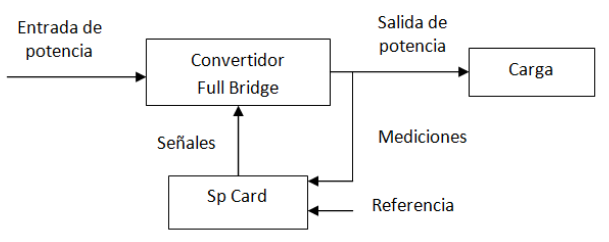
\includegraphics[scale=0.40]{Puente Completo.png}
\caption{Puente Completo }
\label{}
\end{figure}
\subsubsection{Reversible en Tension}
La alimentacion con reversibilidad de tension supondra que la maquina podra girar en ambos sentidos al ser la tension bidireccional, siendo en todo momento el par del mismo signo, al ser la corriente unidireccional.
\subsubsection{Estructuras con aislamiento de mas de un interruptor controlado}
\subsubsection{Push-Pull}
Tiene transistores a la entrada del primario realizando una onda simetrica y diodos en el secundario realizando una rectificación de doble onda.
\subsubsection{Half-Bridge}
Es una simplificacion del Convertidor Puente teniendo en el primario dos transistores y dos condensadores.
\subsubsection{Full-Bridge}
El funcionamiento es igual en el secundario que en el convertidor de Contrafase y el primario realiza la onda simetrica con cuatro transistores en puente trabajando por parejas.


\subsection{Elevador Boost}
El convertidor Boost (o elevador) es un convertidor DC a DC que obtiene a su salida una tensión continua mayor que a su entrada. Es un tipo de fuente de alimentación conmutada que contiene al menos dos interruptores semiconductores (diodo y transistor), y al menos un elemento para almacenar energía (condensador, bobina o combinación de ambos). Frecuentemente se añaden filtros construidos con inductores y condensadores para mejorar el rendimiento. 
\begin{figure}[htp]
\centering
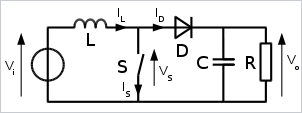
\includegraphics[scale=0.60]{Elevador.png}
\caption{Elevador Boost}
\label{}
\end{figure}
\subsection{Reductor-Elevador}
El convertidor reductor-elevador o tambien conocido como buck-boost suministra un voltaje de salida que puede ser mayor o menor al de la entrada, asi mismo la polaridad del voltaje de salida es inversa a la del voltaje de entrada.\\Un convertidor buck-boost se obtiene por medio de la conexion en cascada de los dos convertidores basicos: el convertidor reductor y el convertidor elevador. En estado permanente la relacion de conversion.
\begin{figure}[htp]
\centering
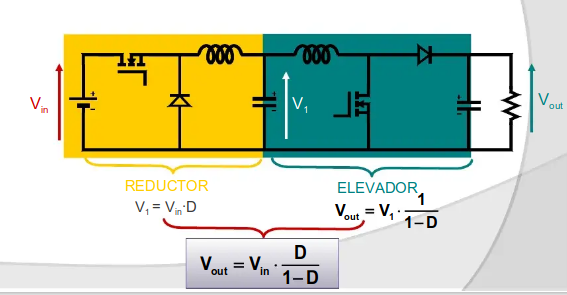
\includegraphics[scale=0.60]{Reductor-Elevador.png}
\caption{Reductor- Elevador}
\label{}
\end{figure}
\subsubsection{De Retroceso (Flyback)}
La salida puede ser de mayor o menor tension que la de entrada pero con la polaridad invertida. Este tipo de convertidor puede ser de salida aislada de la entrada o no. Y en el modelo que está aislado por medio de un transformador puede ser de varias salidas si el transformador es de multiples secundarios.
\pagebreak
\subsubsection{(Flyback) 2 interruptores}
\begin{figure}[htp]
\centering
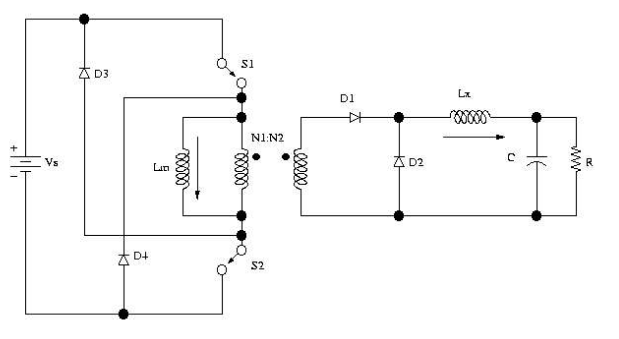
\includegraphics[scale=0.50]{Flyback con 2 interruptores.png}
\caption{Flyback Con 2 Interruptores}
\label{}
\end{figure}
\pagebreak
\subsection{Convertidor de Cuk}
EL cuk Convert es un conversor de voltaje DC-DC, que trabaja tanto como elevador de voltaje como de reductor de voltaje, esto puede influir o no la corriente de salida, siendo este un conversor muy util, este conversor a diferencia de los explicados anteriormente, acumula la energia en los capacitores en vez de inductores, y posee 2 capacitores y 2 inductores. Para estos sistemas tambien podemos aplicar un control para mejorar su funcionamiento, disminuir el tiempo de respuesta, compensar errores en los voltajes de entrada y eliminar sobre-picos ocasionados por la función de transferencia que se utiliza.
\begin{figure}[htp]
\centering
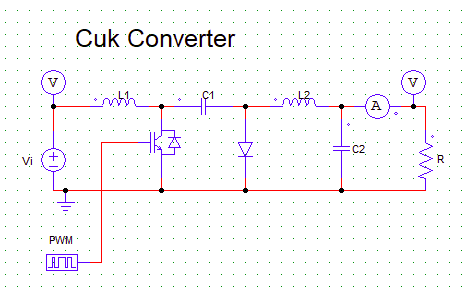
\includegraphics[scale=0.60]{Cuk convert.png}
\caption{Cuk Convert}
\label{}
\end{figure}
\pagebreak


\nocite{*}


\bibliography{ARCHIVOS.TEX.BIB.PDF/Desconocidos2006-2018.bib}{}
\bibliographystyle{plain}
\end{document}
